\documentclass[fleqn, a4paper, 12pt]{article} %untuk soal

\newcommand\mylog[1]{\mathop{{}^{#1}\mathrm{log}}}

\usepackage[textwidth=330px]{geometry}  %untuk soal
\usepackage{amsmath}
\usepackage{amssymb}
\usepackage{graphicx}
\usepackage{color}
\usepackage{hyperref}
\usepackage{tikz}
\usepackage{pst-plot}
\usepackage{multirow}
\usepackage{verbatim}
\usepackage{longtable}
\usepackage{xcolor}
\usepackage{enumerate}
%\usepackage{pgf}
%\usepackage{pgfplots}
\usepackage{multicol}
\usepackage{xfrac}
\hypersetup{
    colorlinks,
    linkcolor={red!50!black},
    citecolor={blue!50!black},
    urlcolor={blue!80!black}
}
	
\title{Sistem Pertidaksamaan Kuadrat - Soal}
\author{Wisnu OPS}

\begin{document}

\maketitle

\tableofcontents

\section{Latihan Soal - PG}

	\begin{enumerate}		
		\item Sistem pertidaksamaan $y \leq 2x^2 + 3x - 1$ dan $y \geq x^2 + 5x + 23$ mempunyai penyelesaian dalam $x$, yaitu ....
		\begin{enumerate}[(A)]
			\item $x \leq -4$ atau $x \geq 6$
			\item $x \leq -6$ atau $x \geq 4$
			\item $x \leq 4$ atau $x \geq 6$
			\item $-4 \leq x \leq 6$
			\item $-6 \leq x \leq 4$			
		\end{enumerate}
		\item Daerah $x$ yang menjadi penyelesaian dari sistem pertidaksamaan $y \leq 2x + 5$ dan $y \geq x^2 - x - 23$ adalah ....
		\begin{enumerate}[(A)]
			\item $x \leq -4$ atau $x \geq 7$
			\item $x \leq -7$ atau $x \geq 4$
			\item $x \leq 4$ atau $x \geq 7$
			\item $-4 \leq x \leq 7$
			\item $-4 \leq x \leq 4$
		\end{enumerate}
		
		\newpage
		
		\item Agar titik $(3, 2)$ merupakan anggota himpunan penyelesaian sistem pertidaksamaan $y \leq 2x^2 + mx - 1$ dan $y \geq x^2 + 2mx + 5$ maka haruslah ....
		\begin{enumerate}[(A)]
			\item $m \leq -2$ atau $m \geq 5$
			\item $m \leq -5$ atau $m \geq -2$
			\item $m \leq 2$ atau $m \geq 5$
			\item $-2 \leq m \leq 5$
			\item $-5 \leq m \leq -2$
		\end{enumerate}
		\item Himpunan penyelesaian dari pertidaksamaan $3x + 4y \leq 12$, $y \geq 0$, dan $y \geq x^2 - 2x -8$ pada gambar di bawah ini menempati daerah ....	\\
			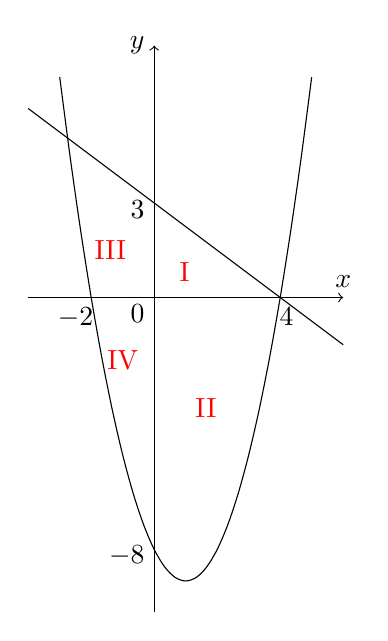
\begin{tikzpicture}[scale=0.4]
				\draw[->] (-4, 0) -- (6, 0) node[above] {$x$};
				\draw[->] (0, -10) -- (0, 8) node[left] {$y$};
				\draw[domain=-3:5, smooth, variable=\x] plot ({\x},{(\x+2)*(\x-4)});
				\draw[domain=-4:6, smooth, variable=\x] plot ({\x},{(-3/4)*\x + 3});
				\draw (0, -0.5) node[left] {$0$};
				\draw (-2.5, 0) node[below] {$-2$};
				\draw (4.2, 0) node[below] {$4$};
				\draw (0, 2.8) node[left] {$3$};
				\draw (0, -8.2) node[left] {$-8$};
				\draw[color=red] (0.5, 0.8) node[right] {I};
				\draw[color=red] (1, -3.5) node[right] {II};
				\draw[color=red] (-2.2, 1.5) node[right] {III};
				\draw[color=red] (-1.8, -2) node[right] {IV};
			\end{tikzpicture}
		\begin{enumerate}[(A)]
			\item I dan II
			\item I dan III
			\item I dan IV
			\item II dan IV
			\item I, II, III, dan IV
		\end{enumerate}
		
		\newpage
		
		\item Daerah yang diarsir pada gambar berikut ini merupakan himpunan penyelesaian dari sistem pertidaksamaan ....	\\
		
			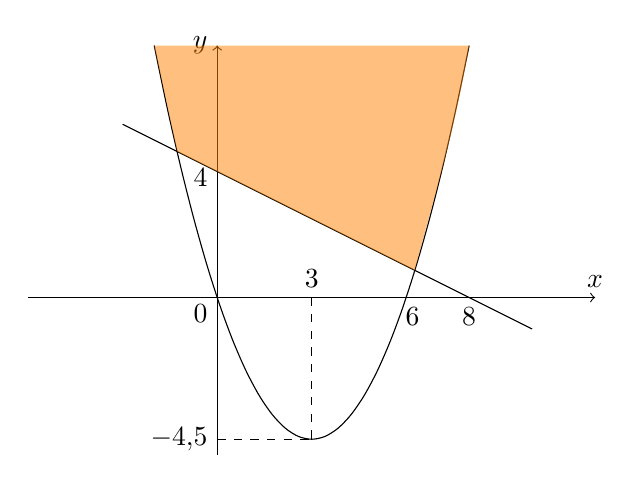
\begin{tikzpicture}[scale=0.4]
				\draw[->] (-6, 0) -- (12, 0) node[above] {$x$};
				\draw[->] (0, -5) -- (0, 8) node[left] {$y$};
				\draw[domain=-2:8, smooth, variable=\x] plot ({\x},{(1/2)*(\x)*(\x-6)});
				\draw[domain=-3:10, smooth, variable=\x] plot ({\x},{(-1/2)*\x + 4});
				\draw (0, -0.5) node[left] {$0$};
				\draw (3, 0) node[above] {$3$};
				\draw (6.2, 0) node[below] {$6$};
				\draw (8, 0) node[below] {$8$};
				\draw (0, -4.5) node[left] {$-4{,}5$};
				\draw (0, 3.8) node[left] {$4$};
				\draw[dashed] (3, 0) -- (3, -4.5);
				\draw[dashed] (0, -4.5) -- (3, -4.5);
				\path[fill=orange, fill opacity=0.5] (6.27, {-6.27/2 + 4}) to [out=75, in=-100] (8, {1/2 * 8 * (8-6)}) -- (-2, {1/2 * (-2) * (-2-6)}) -- (-1.27, {-(-1.27/2) + 4}) -- (6.27, {-6.27/2 + 4});
			\end{tikzpicture}
			
			Note: Nggak tau kenapa di file ini arsirannya nggak transparan. Untuk versi yang transparan, buka file \verb|transparency.pdf|
			
		\begin{enumerate}[(A)]
			\item $y \geq \frac{1}{2}x^2 - 3x$ dan $x + 2y \leq 8$
			\item $y \leq \frac{1}{2}x^2 - 3x$ dan $x + 2y \leq 8$
			\item $y \leq \frac{1}{2}x^2 - 3x$ dan $x + 2y \geq 8$
			\item $y \geq \frac{1}{2}x^2 - 3x$ dan $x + 2y \geq 8$
			\item $y \leq \frac{1}{2}x^2 - 3x$ dan $x + 2y \leq 8$
		\end{enumerate} 
		
		
		
		\newpage
		
		\item Perhatikan gambar berikut:	\\		
			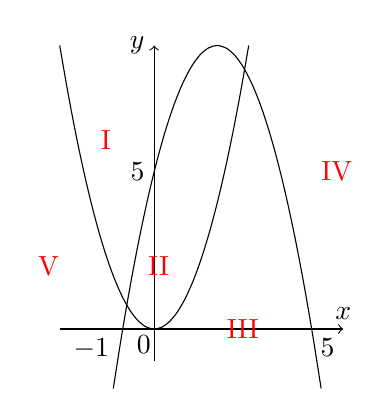
\begin{tikzpicture}[scale=0.4]
				\draw[->] (-3, 0) -- (6, 0) node[above] {$x$};
				\draw[->] (0, -1) -- (0, 9) node[left] {$y$};
				\draw[domain=-1.3:5.3, smooth, variable=\x] plot ({\x},{-(\x)^2+4*\x+5});
				\draw[domain=-3:3, smooth, variable=\x] plot ({\x},{(\x)^2});
				\draw (0.2, -0.5) node[left] {$0$};
				\draw (-2, 0) node[below] {$-1$};
				\draw (5.5, 0) node[below] {$5$};
				\draw (0, 5) node[left] {$5$};
				\draw[color=red] (-2, 6) node[right] {I};
				\draw[color=red] (-0.5, 2) node[right] {II};
				\draw[color=red] (2, 0) node[right] {III};
				\draw[color=red] (5, 5) node[right] {IV};
				\draw[color=red] (-4, 2) node[right] {V};
			\end{tikzpicture}	\\
			Daerah himpunan penyelesaian yang sesuai untuk sistem pertidaksamaan berikut adalah:
			\[\left\{\begin{array}{l}
				-x^2 + 4x - y + 5 \leq 0	\\
				x^2 - y \leq 0
			\end{array}\right.\]
		\begin{enumerate}[(A)]
			\item I
			\item II
			\item III
			\item IV
			\item V
		\end{enumerate}
		
		\newpage
		
		\item Sistem pertidaksamaan yang tepat untuk grafik dengan daerah himpunan penyelesaian pada gambar berikut adalah .... \\
			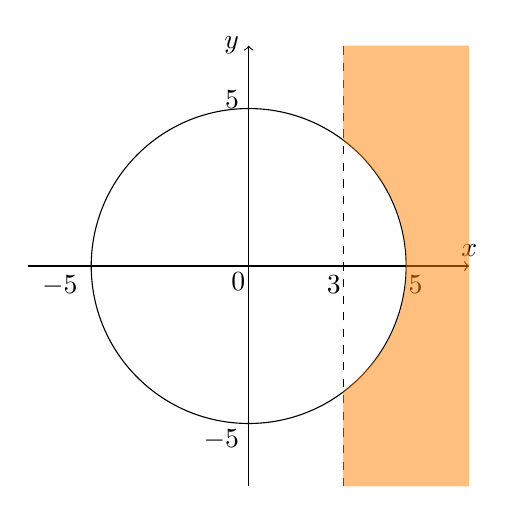
\begin{tikzpicture}[scale=0.4]
				\draw[->] (-7, 0) -- (7, 0) node[above] {$x$};
				\draw[->] (0, -7) -- (0, 7) node[left] {$y$};
				\draw[dashed] (3, -7) -- (3, 7);
				\draw (0.2, -0.5) node[left] {$0$};
				\draw (5.3, 0) node[below] {$5$};
				\draw (0, 5.3) node[left] {$5$};
				\draw (-6, 0) node[below] {$-5$};
				\draw (0, -5.5) node[left] {$-5$};
				\draw (2.7, 0) node[below] {$3$};
				\draw (0, 0) circle (5);
				\path[fill=orange, fill opacity=0.5] (3, 7) -- (3,4) to [out=-40, in=90] (5, 0) to [out=-90, in=40] (3, -4) -- (3, -7) -- (7, -7) -- (7, 7) -- (3, 7);
			\end{tikzpicture}	\\
			
			Note: Nggak tau kenapa di file ini arsirannya nggak transparan. Untuk versi yang transparan, buka file \verb|transparency.pdf|
			
		\begin{enumerate}[(A)]
			\item \[\left\{\begin{array}{l}
					x > 3	\\
					x^2 + y^2 \leq 25	
				\end{array}\right.\]
			\item \[\left\{\begin{array}{l}
					x < 3	\\
					x^2 + y^2 \geq 25	
				\end{array}\right.\]
			\item \[\left\{\begin{array}{l}
					x > 3	\\
					x^2 + y^2 \geq 25	
				\end{array}\right.\]
			\item \[\left\{\begin{array}{l}
					x \geq 3	\\
					x^2 + y^2 \geq 25	
				\end{array}\right.\]
			\item \[\left\{\begin{array}{l}
					x \geq 3	\\
					x^2 + y^2 \leq 25	
				\end{array}\right.\]
				
		\newpage
		
		\end{enumerate}
		\item Yang bukan merupakan penyelesaian dari sistem pertidaksamaan:	\\
			\[\left\{\begin{array}{l}
					y < x^2 + 3x + 2	\\
					y \leq 9 - x^2	
				\end{array}\right.\]
				
			adalah ....
		\begin{enumerate}[(A)]
			\item $(-3, 0)$
			\item $(-2, 0)$
			\item $(-1, -1)$
			\item $(1, 1)$
			\item $(-2, -1)$
		\end{enumerate}
	\end{enumerate}
	
\section{Latihan Soal - Essay}

	Note: Untuk bagian yang ini, nggak semuanya harus dibahas sih. Beberapa soal cuma mengulang konsep yang sama aja. Gue emang bikinnya rada berlebih.

	\begin{enumerate}
		\item Gambarlah himpunan penyelesaian dari sistem pertidaksamaan berikut ini!
			\[\left\{\begin{array}{l}
				y \geq x^2 - 1 \\
				y \leq 4 - x^2
			\end{array}\right.\]
		\item Gambarlah himpunan penyelesaian dari sistem pertidaksamaan berikut ini!
			\[\left\{\begin{array}{l}
				y \geq -x^2 - x + 6	\\
				x + 2y \geq 6	
			\end{array}\right.\]
		\item Gambarlah himpunan penyelesaian dari sistem pertidaksamaan berikut ini!
			\[\left\{\begin{array}{l}
				25 \geq -x^2 - 10y \\
				y \leq x^2 - 25
			\end{array}\right.\]
		\item Gambarlah himpunan penyelesaian dari sistem pertidaksamaan berikut ini!
			\[\left\{\begin{array}{l}
				-x^2 - x - y \leq -2 \\
				-x + y \leq -2
			\end{array}\right.\]	
		\item Gambarlah himpunan penyelesaian dari sistem pertidaksamaan berikut ini!
			\[\left\{\begin{array}{l}
				y \leq x^2 - x - 2 \\
				y \leq 2x^2 - 2x - 4	\\
				y \leq -x^2 + x +2
			\end{array}\right.\]
		\item Gambarlah himpunan penyelesaian dari sistem pertidaksamaan berikut ini!
			\[\left\{\begin{array}{l}
				2y \leq 3x^2 - 27 \\
				y \leq -2x - x^2 \\
				y \leq -x^2 - 5
			\end{array}\right.\]
		\item Gambarlah himpunan penyelesaian dari sistem pertidaksamaan berikut ini!
			\[\left\{\begin{array}{l}
				y \leq -x^2 \\
				y \geq x^2
			\end{array}\right.\]
		\item Gambarlah himpunan penyelesaian dari sistem pertidaksamaan berikut ini!
			\[\left\{\begin{array}{l}
				y \leq -x^2 \\
				y \geq x^2
			\end{array}\right.\]
		\item Gambarlah himpunan penyelesaian dari sistem pertidaksamaan berikut ini!
			\[\left\{\begin{array}{l}
				y \geq 2x^2 + 8 \\
				y \leq -x^2 - 4
			\end{array}\right.\]
	\end{enumerate}

\end{document}